\section{Introduction}

\TODO{Recapitulate main points of project thesis:}

In this chapter, we will study a hypothetical class of compact stars known as quark stars.
Let us summarize the main ingredients in this work.

\subsubsection{The Tolman-Oppenheimer-Volkoff equation}

We will find mass-radius solutions to the Tolman-Oppenheimer-Volkoff equation
\begin{subequations}
\begin{align}
	\odv{P}{r} &= -\frac{G m \epsilon(P)}{r^2 c^2} \left( 1 + \frac{P}{\epsilon(P)} \right) \left( 1 + \frac{4 \pi r^3 P}{m c^2} \right) \left( 1 - \frac{2 G m}{r c^2} \right)^{-1} , \\
	\odv{m}{r} &= \frac{4 \pi r^2 \epsilon(P)}{c^2} ,
\end{align}
\end{subequations}
that we derived in \cref{chap:tov}.
To do so, we integrate it from the center with $m(0) = 0$ and different central pressures $P(0) = P_c$ to the surface defined by $P(R) = 0$ and with corresponding mass $m(R) = M$.

\subsubsection{Equation of state from the grand canonical ensemble}

We will derive equations of state for quark matter by studying effective models of quantum chromodynamics in the zero-temperature approximation.
As we showed in \cref{chap:tft}, the partition function can be calculated as
\begin{equation}
	Z = \trace e^{-\beta (\hat{H} - \mu \hat{N})} = \oint \dif \phi e^{\int_0^\beta \dif \tau \int_V \dif^3 x \, \lagr_E } = e^{-\beta V \Omega} .
\end{equation}
Having found the partition function, we can calculate the
\begin{align}
	\Omega = -\frac{\log Z}{\beta V}, \\
	n = -\pdv{\Omega}{\mu}, \\
	P = -\Omega, \\
	\epsilon = -P + \mu n
\end{align}

\begin{itemize}
\item Tolman-Oppenheimer-Volkoff equation
\item Grand canonical ensemble / partition function: $Z = e^{-\beta V \Omega}$, $n = -\pdv{\Omega}/{\Omega}$, $P = -\Omega$, $\epsilon = -P + \mu n$
\item Charge neutrality and chemical equilibrium (new)
\item Stability/unstability of 2-flavor/3-flavor quark matter (new, for finding bag constant $B$, Bodmer-Witten conjecture)
\end{itemize}

\section{Color confinement, asymptotic freedom and bag models}

(Inspired by \cite{ref:quark_bag_model})

\TODO{discuss $\epsilon$, $P$ before this}

\begin{figure}
\centering
\tikzsetnextfilename{bag-model}
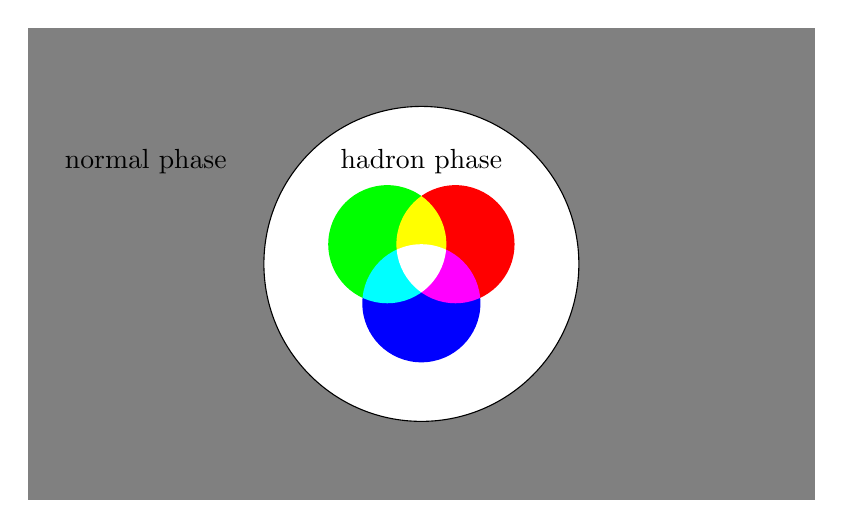
\begin{tikzpicture}
\fill [gray] (-5, -3) rectangle (+5, +3);

\draw [draw=black, fill=white] (0, 0) circle (2);
\begin{scope}[blend group=screen]
	\fill [fill=red]   (30:0.5)  circle (0.75) node {$u$};
	\fill [fill=green] (150:0.5) circle (0.75) node {$d$};
	\fill [fill=blue]  (270:0.5) circle (0.75) node {$s$};
\end{scope}
\node at (90:1.3) {hadron phase};
\node at (-3.5,1.3) {normal phase};
\end{tikzpicture}
\caption{\label{fig:lsm:confinement}%
	\TODO{caption}
}
\end{figure}

\textbf{Color confinement} is a fundamental feature of quantum chromodynamics.
Experiments and lattice simulations have shown that color-charged particles like quarks cannot be isolated from each other, but are rather confined in hadrons.
Quarks can be color-charged \textcolor{red}{\textbf{red}}, \textcolor{green}{\textbf{green}} and \textcolor{blue}{\textbf{blue}},
while antiquarks can have the complementary colors -- or anticolors -- \textcolor{cyan}{\textbf{antired}}, \textcolor{magenta}{\textbf{antigreen}} and \textcolor{yellow}{\textbf{antiblue}}.
For example, a meson consists of one quark of any color and one antiquark with the complementary color of the first quark, making the meson itself \emph{colorless}.
Similarly, a baryon consists of one red, one green and one blue quark,
while an antibaryon consists of one antired, one antigreen and one antiblue quark,
and are thus also colorless.

Another important property of quantum chromodynamics is \textbf{asymptotic freedom}.
As the energy scale of quark interactions increases -- or its length scale decreases -- the \emph{strength} of the interactions \emph{decreases}!
Consequently, 
This property was first discovered by \cite{ref:asymptotic_freedom_gross_wilczek,ref:asymptotic_freedom_politzer} and recognized with the Nobel Prize in 2004.

Together, these two features explain that at high temperature or high density,
quarks become \emph{deconfined} in the sense that they are free of interactions between each other,
but their positions are spatially \emph{confined} to a hadron.
In an extremely dense pure neutron star, for example,
the neutrons' three constituent quarks would break free from each other and hence the bound neutron state due to asymptotic freedom,
but would still be spatially confined to the extent of the original neutron because of color confinement.

To model quark matter and the effect of these two properties,
physicists have come up with various \textbf{bag models}.
As illustrated in \cref{fig:lsm:confinement}, these models split the medium of the physical vacuum state into two phases.
The \emph{normal phase} is the background phase in which quarks are forbidden to exist -- remains of the non-confining medium that existed before the separation into two phases.
On top of the background, bubbles of \emph{hadron phase} are created inside which colorless combinations of quarks are confined.
Mathematically, the confinement is implemented by adding a bag constant $B$ to the grand potential density $\Omega$ of the quarks assumed to live inside the hadronic bubbles.
The bag constant is therefore defined as the energy difference between the hadronic phase and the normal phase,
and creating a hadronic bubble of volume $V$ costs the energy $B V$.
A positive bag constant gives a negative contribution to the pressure $P = -\Omega$,
hence confining the contents of the bag with an external pressure from the surrounding medium in the normal phase.

The \textbf{MIT bag model} is the simplest example.
Consider a star composed of up, down and strange quarks in the zero-temperature and massless approximation.
According to what we learned in \TODO{ref 4.12} and \eqref{eq:nstars:ur_eos}, the grand potential ``before bagging'' is
Pressure
\begin{equation}
	P(\mu) = \smashoperator{\sum_{f=\{u,d,s\}}} \frac{N_c \mu_f^4}{12 \pi^2}
	\qquad \text{and} \qquad
	\epsilon(\mu) = -P(\mu) + \smashoperator{\sum_{f=\{u,d,s\}}} \frac{N_c \mu_f^4}{3 \pi^2}.
\end{equation}
After ``bagging'' the quarks with a bag constant $B$,
\begin{equation}
	P(\mu,B) = P(\mu) - B
	\qquad \text{and} \qquad
	\epsilon(\mu,B) = -P(\mu,B) + \smashoperator{\sum_{f=\{u,d,s\}}} \frac{N_c \mu_f^4}{3 \pi^2}.
	                = -P(\mu,B) + 4 (P(\mu,B) + B) = 4 P(\mu,B) + 4 B.
\end{equation}
The energy density and equation of state is then
\begin{equation}
	\epsilon(P) = -P + \sum_f \mu_f n_f = -P + \sum_f \frac{N_c \mu_f^4}{3 \pi^2} = -P + 4P = 3P
\end{equation}
To ``bag'' the quarks, the idea is 

In the early days of high density and temperature, the universe likely passed through a deconfined quark matter phase.
Today, matter is accreting by nuclear fusion in stars towards iron-56, seemingly representing the ground state of nuclear matter.
However, \cite{ref:strange_hypothesis_bodmer} and \cite{ref:strange_hypothesis_witten} has hypothesized that this state of matter is only \emph{metastable}.
Their \textbf{strange matter hypothesis} claims that the true ground state of nuclear matter is that of three-flavor matter consisting of up, down and strange quarks

\TODO{rewrite?}
We can use the presumed stability of two-flavor and three-flavor quark matter to determine a range of acceptable windows for the bag constant $B$.
Per baryon, iron-56 has an energy of $E/N_B = \epsilon/n_B = \SI{930}{\mega\electronvolt}$,
so if $\epsilon_2$ and $\epsilon_3$ are the energy densities of two-flavor and three-flavor quark matter,
we determine the bag constant $B$ such that
\TODO{at zero pressure?}
\begin{equation}
	\frac{\epsilon_3(0)}{n_B} < \SI{930}{\mega\electronvolt} < \frac{\epsilon_2(0)}{n_B} .
\label{eq:lsm:bag_stability}
\end{equation}
Only the two-flavor bound has been observed,
while the three-flavor bound is a quite reckless assumption that should certainly be taken with a grain of salt.
It will, however, be very useful to have \emph{some} bound for the bag constant in order to constrain the parameter space of equations of state later on.

\TODO{titles}

\TODO{units, $\hbar = c = G = k_B = 1$ or not?}

\TODO{organize project and master thesis together}

\section{Quantum chromodynamics and effective field theory}

\TODO{philosophy of effective field theory: identifty DoF (particles) and symmetries, write down most general Lagrangian with all (relevant) interactions \cite{ref:weinberg_eft}. like small oscillations in classical mechanics?}

\section{Electric charge neutrality and chemical equilibrium in stars}

\TODO{generally, see Halvor's detailed discussion about this}

When we solved the Tolman-Oppenheimer-Volkoff equations for ideal neutron stars in \cref{chap:nstars}, our lives were quite simple.
The stars consisted of only one charge neutral particle, and we simply eliminated its chemical potential to find the equation of state.
Now we will consider stellar models with a greater variety of particles and nonzero electric charge.

How do we now find the equation of state, when there is one chemical potential for each kind of particle?
The answer is to impose additional physical requirements of electric charge neutrality and chemical equilibrium.
With these conditions, we will relate all but one of the chemical potentials to each other, leaving only one independent variable that we will eliminate to find the equation of state.

\subsection{Global electric charge neutrality}

\TODO{could implement this by making EOS $\epsilon(P,r)$ a radial function, and solving $q(r) = f(r)$ for some given $f(r)$? local charge neutrality would then be equal to $f(r) = 0$.}

We can make a very simple classical argument for why there can be no \emph{global} net electric charge in stars by comparing Newton's law of gravity and Coulomb's law.
Consider a test particle of mass $m$ and electric charge $q$ on the surface $R$ from the center of a star with total mass $M$ and electric charge $Q$.
In an idealized situation, the test particle is affected by the gravitational and electrostatic force, so that the total outwards \TODO{radial?} force on it is
\begin{equation}
	F_\text{out} = -G \frac{M m}{R^2} + k_e \frac{Q q}{R^2} .
\end{equation}
Furthermore, suppose the star consists of $N$ particles weighing \TODO{weight $\rightarrow$ mass} no more than some heavy baryon with mass $m_B$, so $M < N M_B$ and $m < m_B$.
Any electrically charged particle has about one elementary charge $q \approx \pm e$.
If the star has an opposite charge $Q = \mp Z e$, then $F_\text{out} < 0$ and the test particle stays in the star.
On the other hand, if the star has a like charge $Q = \pm Z e$, then
\begin{equation}
	F_\text{out} > -G \frac{N m_B^2}{R^2} + k_e \frac{Z e^2}{R^2} .
\end{equation}
We then surely have $F_\text{out} > 0$, provided that the number of elementary charges per particle satisfies
\begin{equation}
	\frac{Z}{N} > \frac{G m_B^2}{k_e e^2} \approx 10^{-37} ,
\end{equation}
where we have assumed a typical baryon mass $m_B = m_p = \SI{1.67e-27}{\kilogram}$.
This corresponds to practically zero electric charge per particle in the star.

This means that particle are expelled from the star while $Z > 10^{-37} N$ until $Z$ has fallen to \emph{at least} $Z < 10^{-37} N$.
We conclude that for all practical purposes, stars are \emph{globally} electrically charge neutral.

\TODO{what about radius $r < R$ instead of $r=R$?}

\TODO{what about general relativity instead of Newtonian gravity?}

\TODO{what about contribution from pressure and other things to $F_\text{out}$?}

\TODO{can I recast inequality in charge per solar mass? see discussion at beginning of \url{www.if.ufrgs.br/hadrons/MMalheiro.pdf}}

\subsection{Local electric charge neutrality}

\TODO{non-understandable comment from Møte 4, Gibbs/Maxwell contstruction etc?}

\TODO{Glendenning has papers regarding local charge neutrality (?)}

The argument in the previous section shows that a star can have no \emph{total} electric charge, but it places absolutely no limitations on its \emph{distribution}.
Moreover, our approach to calculating equations of state is inherently \emph{local} -- we obtain the equation of state $\epsilon(P)$ by eliminating the density $n$ at any \emph{single point} from the energy density $\epsilon(n)$ and pressure $P(n)$.
To make use of electric charge neutrality in our approach, we will promote it from a \emph{global} constraint to a \emph{local} one.

\TODO{now explain...}

\TODO{TOV equation is derived by assuming ideal fluid in equilibrium -- would local charge destroy that?}

\TODO{draw inspiration from standard argument that $\vec{E} = 0$ everywhere inside a conductor?}

Satisfied by
\begin{equation}
	\sum_p q_p \, n(\mu_p) = 0 ,
\label{eq:lsm:charge_neutrality}
\end{equation}
where the sum is over all particles present, each with electric charge $q_p$.
In the zero-temperature approximation with the density \eqref{eq:nstars:density_zeroT}, this is satisfied if
\begin{equation}
	\sum_p q_p \left( \mu_p^2 - m_p^2 \right)^{3/2} = 0 .
\end{equation}

\subsection{Chemical equilibrium}

\TODO{introduce}

Important reactions
\begin{subequations}
\begin{align}
	d     &\leftrightarrow u + e + \bar{\nu}_e, \\
	s     &\leftrightarrow u + e + \bar{\nu}_e, \\
	s + u &\leftrightarrow u + d .
\end{align}
\end{subequations}
Assume neutrinos leave star \TODO{why?}.
Then chemical equilibrium implies
\begin{subequations}
\begin{align}
	\mu_d &= \mu_u + \mu_e, \\
	\mu_s &= \mu_u + \mu_e, \\
	\mu_s &= \mu_d .
\end{align}
\label{eq:lsm:chemical_equilibrium}
\end{subequations}
(the third follows automatically from the two first)

\subsection{Symmetries}

Always have $U(1)_V$ symmetry, giving rise to conservation of baryon number.

Symmetry breaking
\begin{equation}
	SU(2)_L \times SU(2)_R \quad \rightarrow \quad SU(2)_V
\end{equation}
Quark-meson model can be written in terms of left/right fields:
\begin{equation}
\begin{split}
	\bar{\psi} \phi_5 \psi &= \bar{\psi} ( (P_+ + P_-) \sigma + (P_+ - P_-) i \tau \cdot \pi) \psi \\
	                       &= \bar{\psi} ( P_+ (\sigma + i \tau \cdot \pi) + P_- (\sigma - i \tau \cdot \pi) ) \psi \\
	                       &= \bar{\psi} ( P_+ \phi + P_- \phi^\dagger) \psi \\
	                       &= \bar{\psi} ( P_+ \phi P_+ + P_- \phi^\dagger P_-) \psi \\
	                       &= \bar{\psi}_- \phi P_+ + \bar{\psi}_+ \phi^\dagger \psi_- \\
\end{split}
\end{equation}
Used that $P_\pm^2 = P_\pm$ is in spinor-space, while $\phi$ is in flavor space.
Denote $+ = R$, $- = L$.
Now it is apparent that LSM is invariant under $SU(2)_L \times SU(2)_R$:
\begin{equation}
	\psi_+ \rightarrow U_+ \psi_+, \qquad
	\psi_- \rightarrow U_- \psi_-, \qquad
	\phi   \rightarrow U_- \phi U_+^\dagger.
\end{equation}
When $h \neq 0$, this symmetry is explicitly broken.



